
%%%%%%%%%%%%%%%%%%%%%%%%%%%%%%%%%%%%%%%%%
% Jacobs Landscape Poster
% LaTeX Template
% Version 1.0 (29/03/13)
%
% Created by:
% Computational Physics and Biophysics Group, Jacobs University
% https://teamwork.jacobs-university.de:8443/confluence/display/CoPandBiG/LaTeX+Poster
% 
% Further modified by:
% Nathaniel Johnston (nathaniel@njohnston.ca)
%
% Modified further still by:
% Abraham Nunes (nunes <at> dal <dot> ca)
%
% License:
% CC BY-NC-SA 3.0 (http://creativecommons.org/licenses/by-nc-sa/3.0/)
%
%%%%%%%%%%%%%%%%%%%%%%%%%%%%%%%%%%%%%%%%%

%----------------------------------------------------------------------------------------
%	PACKAGES AND OTHER DOCUMENT CONFIGURATIONS
%----------------------------------------------------------------------------------------

\documentclass[final]{beamer}

\usepackage[scale=1.24]{beamerposter} % Use the beamerposter package for laying out the poster

\usetheme{confposter} % Use the confposter theme supplied with this template

\setbeamercolor{block title}{fg=black,bg=white} % Colors of the block titles
\setbeamercolor{block body}{fg=black,bg=white} % Colors of the body of blocks
\setbeamercolor{block alerted title}{fg=white,bg=erd} % Colors of the highlighted block titles
\setbeamercolor{block alerted body}{fg=black,bg=white} % Colors of the body of highlighted blocks
% Many more colors are available for use in beamerthemeconfposter.sty

%-----------------------------------------------------------
% Define the column widths and overall poster size
% To set effective sepwid, onecolwid and twocolwid values, first choose how many columns you want and how much separation you want between columns
% In this template, the separation width chosen is 0.024 of the paper width and a 4-column layout
% onecolwid should therefore be (1-(# of columns+1)*sepwid)/# of columns e.g. (1-(4+1)*0.024)/4 = 0.22
% Set twocolwid to be (2*onecolwid)+sepwid = 0.464
% Set threecolwid to be (3*onecolwid)+2*sepwid = 0.708
\usepackage[english,russian]{babel}
\usepackage[utf8]{inputenc}
\usepackage{mwe}
\newlength{\sepwid}
\newlength{\onecolwid}
\newlength{\twocolwid}
\newlength{\threecolwid}
\setlength{\paperwidth}{48in} % A0 width: 46.8in
\setlength{\paperheight}{36in} % A0 height: 33.1in
\setlength{\sepwid}{0.024\paperwidth} % Separation width (white space) between columns
\setlength{\onecolwid}{0.22\paperwidth} % Width of one column
\setlength{\twocolwid}{0.464\paperwidth} % Width of two columns
\setlength{\threecolwid}{0.708\paperwidth} % Width of three columns
\setlength{\topmargin}{-0.5in} % Reduce the top margin size
%-----------------------------------------------------------

\usepackage{graphicx}  % Required for including images

\usepackage{booktabs} % Top and bottom rules for tables

%----------------------------------------------------------------------------------------
%	TITLE SECTION 
%----------------------------------------------------------------------------------------

\title{Энтропия} % Poster title

\author{Терверессы: Лиза, Олеся, Даша, Марина, Яна} % Author(s)
\titlegraphic{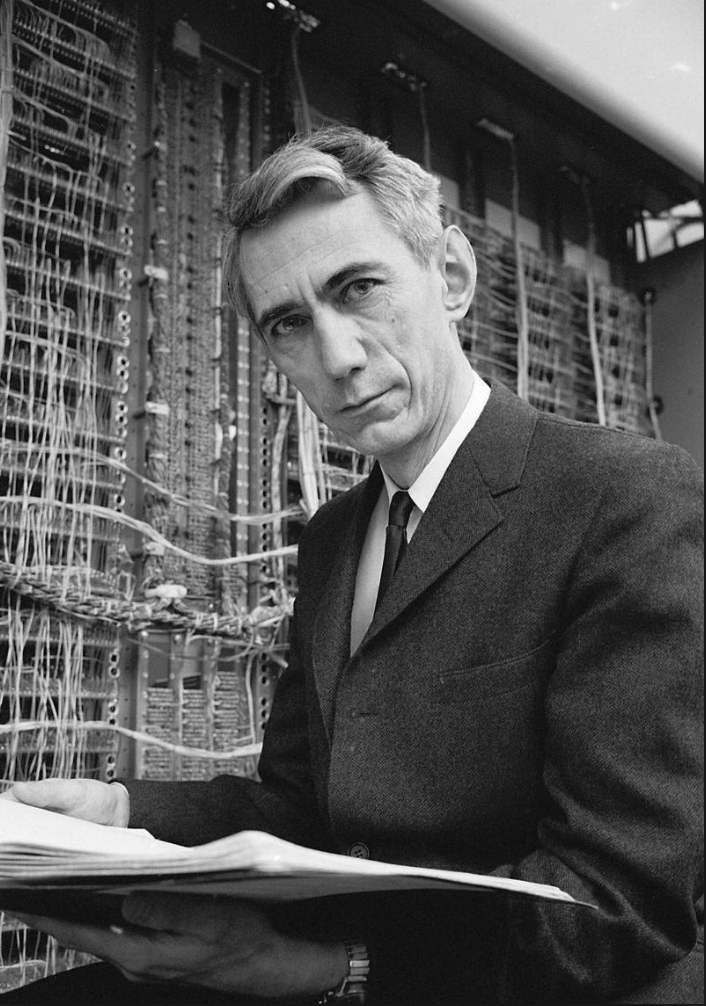
\includegraphics[scale=0.5]{klod.png}}
\institute{БЭК 171} % Institution(s)


%----------------------------------------------------------------------------------------

\begin{document}

\addtobeamertemplate{block end}{}{\vspace*{2ex}} % White space under blocks
\addtobeamertemplate{block alerted end}{}{\vspace*{2ex}} % White space under highlighted (alert) blocks

\setlength{\belowcaptionskip}{2ex} % White space under figures
\setlength\belowdisplayshortskip{2ex} % White space under equations

\begin{frame}[t] % The whole poster is enclosed in one beamer frame

\begin{columns}[t] % The whole poster consists of three major columns, the second of which is split into two columns twice - the [t] option aligns each column's content to the top

\begin{column}{\sepwid}\end{column} % Empty spacer column

\begin{column}{\onecolwid} % The first column

%----------------------------------------------------------------------------------------
%	OBJECTIVES
%----------------------------------------------------------------------------------------

\setbeamercolor{block alerted title}{fg=white,bg=jblue} % Change the alert block title colors
\setbeamercolor{block alerted body}{fg=black,bg=white} % Change the alert block body colors

\begin{alertblock}{Откуда появилась?}
% Очень кратко, тезисно, написать про историю энтропии (сжать исходный текст)
    \begin{itemize}
    \item 1948 год - Клод Шеннон создал первую, истинно математическую, теорию энтропии
    \item Его идеи послужили основой разработки двух основных направлений: \textit{теории информации} и \textit{теории кодирования}
    \end{itemize}
    
    \end{alertblock}
%----------------------------------------------------------------------------------------
%	INTRODUCTION
%----------------------------------------------------------------------------------------

\begin{block}{Для дискретных случайных величин}

\begin{itemize}
    \item 
\end{itemize}

\textbf{Пример.} Текст задачи
\end{block}

\begin{alertblock}{Свойства}
	% Очень кратко, тезисно, написать про историю энтропии (сжать исходный текст)
	\begin{itemize}
		\item 
	\end{itemize}
	
\end{alertblock}

\begin{block}{Кросс-энтропия и дивергенция Кульбака-Лейблера}
	\begin{itemize}
		\item 
	\end{itemize}

\textbf{Пример.} Текст задачи
\end{block}

%------------------------------------------------

%\begin{figure}
%\includegraphics[width=0.8\linewidth]{placeholder.jpg}
%\caption{Figure caption}
%\end{figure}

%----------------------------------------------------------------------------------------

\end{column} % End of the first column

\begin{column}{\sepwid}\end{column} % Empty spacer column

\begin{column}{\twocolwid} % Begin a column which is two columns wide (column 2)

\begin{columns}[t,totalwidth=\twocolwid] % Split up the two columns wide column

\begin{column}{\onecolwid}\vspace{-.6in} % The first column within column 2 (column 2.1)

%----------------------------------------------------------------------------------------
%	MATERIALS
%----------------------------------------------------------------------------------------

\begin{block}{Для непрерывных случайных величин}

\begin{itemize}
\item Curabitur pellentesque dignissim
\item Eu facilisis est tempus quis
\item Duis porta consequat lorem
\item Eu facilisis est tempus quis
\end{itemize}


\begin{enumerate}
\item Curabitur pellentesque dignissim
\item Eu facilisis est tempus quis
\item Duis porta consequat lorem
\item Curabitur pellentesque dignissim
\end{enumerate}

\textbf{Пример.} Текст задачи
\end{block}

%----------------------------------------------------------------------------------------

\end{column} % End of column 2.1

\begin{column}{\onecolwid}\vspace{-.6in} % The second column within column 2 (column 2.2)

%----------------------------------------------------------------------------------------
%	METHODS
%----------------------------------------------------------------------------------------

\begin{block}{Применение}
\textbf{Энтропийное кодирование}

%\begin{figure}
%\includegraphics[width=0.8\linewidth]{placeholder.jpg}
%\caption{Figure caption}
%\end{figure}

Энтропия показывает наименьшее среднее число бит, необходимое для кодирования некоторой информации. С целью минимизации энтропии и оптимизации кода элементы с большой вероятностью появления кодируются меньшим числом символов. Это позволяет передавать большее количество информации, затрачивая меньший объем памяти.

\textbf{Построение решающих деревьев}

Каждое ветвление дерева представляет собой разделение выборки на две части по порогу некоторого признака. Расчет энтропии помогает определить оптимальный порог для каждого узла --- при котором взвешенная сумма энтропий получившихся выборок минимальна среди возможных разбиений.

Например, у нас есть выборка объектов с одним признаком, длина: обыкновенный удав (22 попугая), анаконда (46 попугаев), анаконда (40 попугаев), обыкновенный удав (31 попугай).

Попробуем разделить выборку по 38 попугаям:
\begin{center}
	\tikzstyle{level 1}=[level distance=2cm, sibling distance=7cm]
	\tikzstyle{level 2}=[level distance=2cm, sibling distance=1cm]
	\tikz
	\node {Длина < 38 попугаев}
	child { node {Да}
		child { node {Обыкновенный удав, обыкновенный удав}}}
	child { node {Нет}
		child { node {Анаконда, анаконда}}};
\end{center}

При расчете энтропии $0 \cdot \log_2 0$ считается равным 0, несмотря на $\log_2 0$. За вероятность принимается вероятность встретить данный класс в новой выборке.

Энтропия левой части: $-(1 \cdot \log_2 1 + 0 \cdot \log_2 0) = 0$. Энтропия правой части: $-(1 \cdot \log_2 1 + 0 \cdot \log_2 0) = 0$. Суммарная энтропия получилась: $\frac{1}{2} \cdot 0 + \frac{1}{2} \cdot 0 = 0, \frac{1}{2}$ --- доля каждой выборки в исходной. 

Так как 0 --- минимально возможное значение энтропии, критерий <<длина < 38 попугаев>> дает оптимальный результат.
\end{block}

%----------------------------------------------------------------------------------------

\end{column} % End of column 2.2

\end{columns} % End of the split of column 2 - any content after this will now take up 2 columns width

%----------------------------------------------------------------------------------------
%	IMPORTANT RESULT
%----------------------------------------------------------------------------------------

\setbeamercolor{block alerted title}{fg=black,bg=dalgold} % Change the alert block title colors
\setbeamercolor{block alerted body}{fg=black,bg=white} % Change the alert block body colors

%----------------------------------------------------------------------------------------

\begin{columns}[t,totalwidth=\twocolwid] % Split up the two columns wide column again

\begin{column}{\onecolwid} % The first column within column 2 (column 2.1)

%----------------------------------------------------------------------------------------
%	MATHEMATICAL SECTION
%----------------------------------------------------------------------------------------

%----------------------------------------------------------------------------------------

\end{column} % End of column 2.1

\begin{column}{\onecolwid} % The second column within column 2 (column 2.2)

%----------------------------------------------------------------------------------------
%	RESULTS
%----------------------------------------------------------------------------------------



%----------------------------------------------------------------------------------------

\end{column} % End of column 2.2

\end{columns} % End of the split of column 2

\end{column} % End of the second column

\begin{column}{\sepwid}\end{column} % Empty spacer column

\begin{column}{\onecolwid} % The third column

%----------------------------------------------------------------------------------------
%	CONCLUSION
%----------------------------------------------------------------------------------------

\textbf{Применение в алгоритме UMAP}

В анализе данных алгоритмы снижения размерности используют кросс-энтропию как показатель эффективности перенесения свойств объектов. Чем меньше кросс-энтропия, тем ближе к истинному оказалось подобранное отображение.

Приведем пример работы алгоритма UMAP. Мы возьмем набор данных об одежде, который включает в себя 70000 черно-белых изображений различной одежды по 10 классам: футболки, брюки, свитеры, платья, кроссовки и т.д. Каждая картинка имеет размер 28x28 пикселей или 784 пикселя.

Результатом преобразования будет следующее отображение:

\begin{figure}[!h]
	\noindent\centering{
		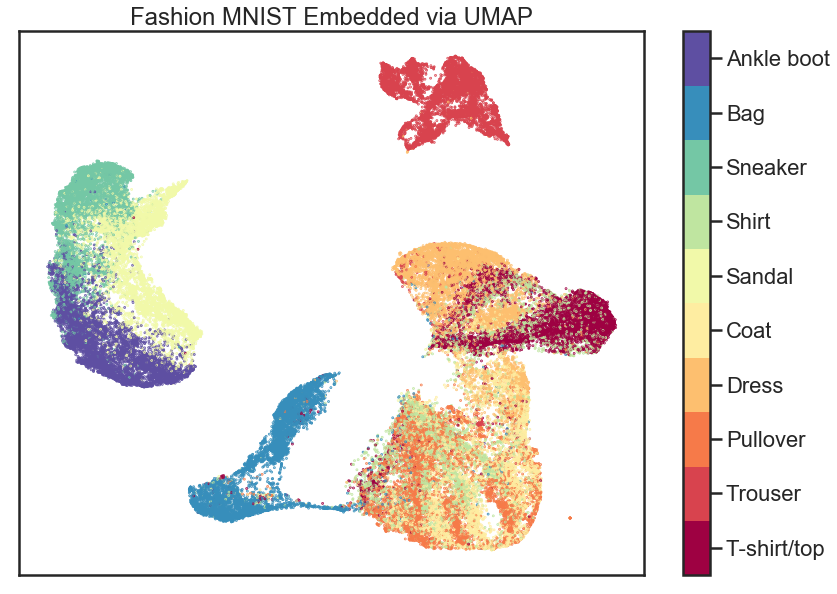
\includegraphics[height=9cm]{umap.png}
	}
	\caption{Алгоритм UMAP}
	\label{figCurves}
\end{figure} 

Для оптимального подбора признаков в UMAP используется дивергенция Кульбака-Лейблера для случайной величины Бернулли $X \sim B(p(x))$:
\[D_{KL}(P\, ||\, \tilde P)= - p(x)\log \tilde p(x) - (1 - p(x))\log (1 - \tilde p(x)) + p(x)\log p(x) + (1 - p(x))\log (1 - p(x)) = \]
\[= p(x)\log \frac{p(x)}{\tilde p(x)} + (1 - p(x))\log \frac{1 - p(x)}{1 - \tilde p(x)}\]

Однако алгоритм рассчитывает не просто разницу между двумя распределениями для одной случайной величины, а сумму таких разниц для $n$ случайных величин:
\[S(P||\tilde P) = \sum_{i=1}^n p(x_i)\log \frac{p(x_i)}{\tilde p(x_i)} + (1 - p(x_i))\log \frac{1 - p(x_i)}{1 - \tilde p(x_i)}\]

Данная величина показывает степень отдаленности друг от друга множеств из случайных величин: $P$ и $\tilde P$. Минимизация $S(P||\tilde P)$ по $\tilde p(x)$ позволяет найти множество $\tilde P$, которое наиболее похоже на множество $P$.

Задача минимизации заключается в поиске оптимального $\tilde p(x)$. Если вернуться к исходной записи $D_{KL} = CE(P||\tilde P) - H(p)$, то видно, что энтропия не зависит от $\tilde p(x)$, соответственно, является константой при минимизации. Тогда задача преобразуется в оптимизацию лишь суммы кросс-энтропий:
\[- \sum_{i=1}^n \left(p(x_i)\log \tilde p(x_i) + (1 - p(x_i))\log (1 - \tilde p(x_i))\right) \rightarrow \min_{\tilde p}\]

Поэтому UMAP считается методом, основанным на кросс-энтропии.

При отображении пространстве UMAP строит взвешенный граф из объектов. Веса ребер можно воспринимать как вероятность существования данного ребра. Поэтому ребро $e$ является случайной величиной, имеющей распределение Бернулли: $e \sim B(w(e))$, где $w(e)$ --- вес ребра $e$. Получается, что множество ребер построенного графа --- множество $E$ из случайных величин Бернулли.

Тогда для более корректного переноса данных мы можем подобрать для множества~$E_h$ похожее на него множество~$E_l$ с функцией~$w_l(e)$, соответствующие низкоразмерному пространству.

%----------------------------------------------------------------------------------------
%	ADDITIONAL INFORMATION
%----------------------------------------------------------------------------------------

%----------------------------------------------------------------------------------------
%	ACKNOWLEDGEMENTS
%----------------------------------------------------------------------------------------

\setbeamercolor{block title}{fg=black,bg=white} % Change the block title color


%----------------------------------------------------------------------------------------
%	CONTACT INFORMATION
%----------------------------------------------------------------------------------------

\setbeamercolor{block alerted title}{fg=black,bg=dalblue} % Change the alert block title colors
\setbeamercolor{block alerted body}{fg=black,bg=white} % Change the alert block body colors

\begin{alertblock}{Contact Information}

\begin{itemize}
\item Web: http://www.YourWebsite.com/lab
\item Email: youremail@emailprovider.com
\end{itemize}

\end{alertblock}

%\begin{center}
%\includegraphics[width=0.8\linewidth]{dal_fullmark_blak.jpg}
%\end{center}
%----------------------------------------------------------------------------------------

\end{column} % End of the third column

\end{columns} % End of all the columns in the poster

\end{frame} % End of the enclosing frame

\end{document}